\subsection{A Polynomial Time Algorithm For Solving \mainproblem}\label{sect:st-dPaths}

\begin{algorithm}[t]
\caption{Solving the \texttt{\mainproblem} problem.}\label{ALGO:solve}
\DontPrintSemicolon
\nonl \SetKwProg{Fn}{Procedure}{}{}
\footnotesize
\Fn{}{
\KwIn{an instance  of \mainproblem.}
\KwOut{a pair  where the path  is
a solution to {\mainproblem} if such a path exists, \texttt{NO} otherwise.}
; \label{algo:solve:l1} \hfill\tcp{let  be the distance between  and }
; ; \label{algo:solve:l2}
                \tcp{init the \emph{frontier}  and its \emph{level counter}  }
; ; \label{algo:solve:l3}
                \tcp{init the \emph{frontier}  and its \emph{level counter}  }
\While{\texttt{TRUE}}{ \label{algo:solve:l4}
    ; \label{algo:solve:l5} \;
    \If{  \texttt{ OR }  \texttt{ OR }
                ( \texttt{ AND } )}{ \label{algo:solve:l6}
    \Return{\texttt{NO}}; \label{algo:solve:l7}
    }
    \If{  \texttt{ AND }  }{ \label{algo:solve:l8}
        ; \label{algo:solve:l9} \;
        \Return{}; \label{algo:solve:l10}
    }
    ; \label{algo:solve:l11} \;
    \lIf{}{\Return{};} \label{algo:solve:l12}
    \lElse{;} \label{algo:solve:l13}
}
}
\end{algorithm}
We now describe a polynomial time algorithm for solving {\mainproblem}, called
\texttt{solve\_\mainproblem()}, which
takes as input an instance  of \mainproblem, and
returns a pair  where  is a directed path in  that goes from source  to target 
avoiding  if such a path exists (otherwise, the algorithm simply returns \texttt{NO}).
Algorithm~\ref{ALGO:solve} shows the pseudocode for that procedure.
The rationale at the base of \texttt{solve\_\mainproblem()} consists in the continuous iteration of two major phases:
\texttt{double-bfs\_phase()} (line~\ref{algo:solve:l5})
and
\texttt{compression\_ phase()} (line~\ref{algo:solve:l11}).
Throughout computation, both phases alternate repeatedly
until a final state of termination is eventually reached
(either at line~\ref{algo:solve:l7}, line~\ref{algo:solve:l10} or line~\ref{algo:solve:l12}).
At that point, the algorithm either returns a pair  where  is the sought directed path, or a negative response \texttt{NO} instead.
We now describe both phases in more detail, and give the corresponding pseudocode.

\paragraph{Breadth-First Search phases}
The first search  starts from the source vertex  and moves upward,
from lower to higher levels of .
Meanwhile, it collects a certain (polynomially bounded) amount of vertices that do not lie in .
In particular, at the end of any  phase,
the number of collected vertices will always
lie between  and 
(see line~\ref{algo:bfs:l1} of \texttt{bfs\_phase()}).
The set  of vertices collected at the end of  is called the \emph{(source) frontier} of .
All vertices within  have the same cardinality, \ie  for every .
Also, the procedure keeps track of the highest level of depth  that is reached during .
Thus,  corresponds to the distance between the source vertex  and
the current frontier ,
formally,  for every .
Since at the beginning of the computation  starts from the source vertex ,
\texttt{solve\_\mainproblem()} initializes  to  and  to  at line~\ref{algo:solve:l2}.

\begin{algorithm}[t]
\caption{Breadth-First-Search phases.}\label{ALGO:double_bfs}
\DontPrintSemicolon
\SetKwProg{Fn}{Procedure}{}{}
\footnotesize
\nonl\Fn{\texttt{double-bfs\_phase}}{
\setcounter{AlgoLine}{0}

; \label{algo:two_bfs:l1} \tcp{}
; \label{algo:two_bfs:l2} \tcp{}
\Return{}; \label{algo:two_bfs:l3} \;
}

\SetKwProg{SubFn}{SubProcedure}{}{}
\nonl\SubFn{\texttt{\textbf{bfs\_phase}}}{
\setcounter{AlgoLine}{0}

\While{  }{ \label{algo:bfs:l1}
	; \label{algo:bfs:l2} \;
	; \label{algo:bfs:l3} \;
}
\Return{}; \label{algo:bfs:l4}
}

\setcounter{AlgoLine}{0}

\nonl\SubFn{}{
\setcounter{AlgoLine}{0}
; \label{algo:next_bfs:l1} \;
\ForEach{}{ \label{algo:next_bfs:l2}
	;\hfill\tcp{ is  if , otherwise it is  \label{algo:next_bfs:l3}}
}
\Return{}; \label{algo:next_bfs:l4}
}
\end{algorithm}

Similarly, the second search  starts from the target vertex  and moves downward,
from higher to lower levels of , also collecting a certain (polynomially bounded) amount of vertices that do not lie in .
As in the previous case, this amount will always
lie between  and .
The set  of vertices collected at the end of 
is called the \emph{(target) frontier} of .
All vertices within  have the same cardinality.
Also, the procedure keeps track of the \emph{lowest} level of depth  that  has reached.
Thus,  corresponds to the \emph{distance} between the target vertex  and the frontier ,
so that  for every . Since at the beginning of the computation,
 starts from the target vertex ,
\texttt{solve\_\mainproblem()} initializes  and  at line~\ref{algo:solve:l3}.
\figref{fig:double_bfs_phase} provides an illustration of the behaviour of \texttt{double-bfs\_phase()}.

In summary, after any round of \texttt{double-bfs\_phase()}, we are left with two (possibly empty) frontier sets  and .
In Algorithm~\ref{ALGO:solve}, whenever  or  holds at line~\ref{algo:solve:l6},
then at least one frontier set could not proceed one level further in  while avoiding ,
and thus the procedure halts by returning \texttt{NO} at line~\ref{algo:solve:l7}.
Similarly, whenever  and  holds at line~\ref{algo:solve:l6},
the computation halts by returning \texttt{NO} at line~\ref{algo:solve:l7} --- the underlying intuition being that
 and  have finally reached one another's level of depth without intersecting each other,
which means that  contains no directed path from  to  that avoids .

\begin{figure}[htbp]
\centering
\begin{tikzpicture}[baseline= (a).base]
\node[scale=1] (a) at (0,0){
\begin{tikzcd}[
  every arrow/.append style={-,thick},
  matrix of math nodes maybe/.append style={/tikz/cells={/tikz/nodes={/tikz/draw,/tikz/shape=circle,align=center,text width=\widthof{}}}},
  row sep=normal,
  column sep=large,
  thick,
  ]
        & 1,2,3 \dar \dlar \drar  \dar[shift left=.25cm, shorten=.1cm, -stealth]\\
\textit{\textbf{1,2}} & 1,3      \dlar \drar  & \textit{\textbf{2,3}} \\
 1 \uar
        &    \textit{\textbf{2}}         \ular \urar &   \textit{\textbf{3}} \uar\\
        & \emptyset \uar \ular \urar \ular[shift left=.25cm, shorten=.25cm, -stealth]
\end{tikzcd}
};
\end{tikzpicture}
\caption{A \texttt{double\_bfs\_phase()} on  that starts from  and .
The forbidden vertices are ,
 while the edges explored by  and
 are  and  (respectively).}\label{fig:double_bfs_phase}
\end{figure}

On the other
hand,
if both  and
 hold at line~\ref{algo:solve:l8},
then we can prove that for
every , there exists at least one directed path in 
that goes from the source  to  avoiding .
Similarly, for every , there exists at least one directed
path in  that goes from  to target  avoiding .
Therefore, whenever , the algorithm is in the right position to reconstruct
a directed path  in  that goes
from source  to  and from  to target  avoiding  (line~\ref{algo:solve:l9}).
In practice, the reconstruction can be implemented by maintaining a \texttt{map}
throughout the computation, which associates to every vertex  (possibly visited during the BFSs)
the \emph{parent vertex}, , which
led to discover  first.
As soon as  gets constructed,
\texttt{solve\_\mainproblem()} returns 
at line~\ref{algo:solve:l10},
and the computation halts.

\paragraph{Compression Phase}
After \texttt{double-bfs\_phase()} has completed,
the procedure \texttt{solve\_\mainproblem()} also needs to handle
the case
where  and .
The phase that starts at that point is named \texttt{compression\_phase()}
(see Algorithm~\ref{ALGO:compression_phase}).
\begin{algorithm}[t]
\caption{Compression phase.}\label{ALGO:compression_phase}
\nonl\SetKwProg{Fn}{Procedure}{}{}
\DontPrintSemicolon
\footnotesize
\Fn{}{
	; \label{algo:compression:l1} \;
	\While{\texttt{TRUE}}{ \label{algo:compression:l2}
		; \label{algo:compression:l3}\;
		; \label{algo:compression:l4}\;
		\If{}{ \label{algo:compression:l5}
    		  ; \label{algo:compression:l6}\;
		  ; \label{algo:compression:l7}\;
		  ; \label{algo:compression:l8}\;
			; \label{algo:compression:l9} \;
			\Return{}; \label{algo:compression:l10}
		}
		; \label{algo:compression:l11}\;
		; ; \label{algo:compression:l12}\;
		; \label{algo:compression:l13}\;
		; \label{algo:compression:l14} \;
		\If{  \texttt{ OR } (
						\texttt{ AND }  )}{ \label{algo:compression:l15}
			\Return{}; \label{algo:compression:l16}
		}
		\If{ 
				\texttt{ AND }  }{ \label{algo:compression:l17}
			; \label{algo:compression:l18} \;
			\Return{}; \label{algo:compression:l19}
		}
	}
}
\end{algorithm}
This procedure takes as input a tuple
,
where  and  are the current frontier sets.
Recall that  holds due to line~\ref{algo:bfs:l1} of \texttt{bfs\_phase()}.
Also,  is the set of forbidden vertices;
 is the level counter of  and  is that
of ; finally  is the distance between the source  and the target , and  is the size of the ground set.
The output returned by \texttt{compression\_phase()} is either a path  going from source  to target 
avoiding  \texttt{or} a subset  such that the following two basic properties hold:


(1) , and
(2) if  is any directed path in  going from
 to  avoiding , then  goes from  to .


This frontier set  is dubbed the \emph{compression} of . The underlying rationale goes as follows.
On one hand, because of (1), it is possible to keep the search going on by applying yet another round of \texttt{double-bfs\_phase()} on input  and 
(in fact, the size of  has been compressed down to ,
thus matching the threshold condition ``" checked at line~1 of \texttt{bfs\_phase()}).
On the other hand, because of (2), it is indeed sufficient to seek for a directed path in  that goes from  to  avoiding ,
namely, the search can actually forget about  because it leads to a dead end.
\begin{figure}[!htb]
    \centering
    \begin{tikzpicture}[scale=.68, level distance=35pt,sibling distance=9pt]
    \Tree [. \framebox{}
        \edge node[left, xshift=-1ex]{};
    [. \framebox{}
     \edge node[left,xshift=-1ex]{};
     [. \framebox{}
        \edge node[left, xshift=-1ex]{};
        [. \framebox{}
            \edge node[]{};
            [. \framebox{}
                \edge node[left, xshift=-1ex]{};
                [. \framebox{}
                    \edge node[left, xshift=-.25ex, yshift=1ex]{};
[. \framebox{}
                        \edge node[left, xshift=-1ex]{};
                            [. \framebox{}
                            ]
                        \edge node[right, xshift=1ex]{};
                        [. \framebox{}
                        ]
                        ]
]
                \edge node[right, xshift=1ex]{};
                    [. \framebox{}
                    ]
            ]
        ]
        \edge node[right, xshift=1ex]{};
        [. \framebox{}
        ]
     ]
    ]
    \edge node[right, xshift=1ex]{};
    [. \framebox{} ]
    ]
    \end{tikzpicture}
    \caption{The frontier sets of the \texttt{compression\_phase()}.}
\label{fig:compression_phase}
\end{figure}
We now describe \texttt{compression\_phase()} in more details,
and give a graphical summary in \figref{fig:compression_phase}.
The procedure repeatedly builds an undirected bipartite graph
,
where  and
every vertex
 is adjacent to a vertex 
if and only if .
It then uses the procedure \texttt{compute\_max\_matching()} to find a matching
 of size ,
  where  denotes the size of a maximum cardinality matching of .
Notice that the following holds due to line~\ref{algo:bfs:l1} of :

thus, we have the following bound on the size of its edge set:


\begin{algorithm}[t]
\caption{Self-Reduction for computing .}\label{ALGO:self_reduction}
\nonl\SetKwProg{Fn}{Procedure}{}{}
\DontPrintSemicolon
\footnotesize
\Fn{}{
;\label{algo:self-red:l1}\;
  \lIf{}{
      \Return{;\label{algo:self-red:l2}}
    }
     pick one vertex  having maximum degree  in ;\label{algo:self-red:l3}\;
    \If{\label{algo:self-red:l4}}{
       compute a matching  of  s.t. , with the Hopcroft-Karp's algorithm~\cite{HK73};\label{algo:self-red:l5}\;
    }
    \If{\label{algo:self-red:l6}}{
       remove  from ; and call the resulting graph ;\label{algo:self-red:l7}\;
      ;\label{algo:self-red:l8}\;
       there must be at least one edge  such that  is not matched in ,
      therefore, add  to ; and assign the resulting matching to ;\label{algo:self-red:l9}\;
    }
    \Return{;\label{algo:self-red:l10}}
}
\end{algorithm}

The fact is that, given that we are content with a cardinality matching of size at most ,
it is worth applying the following recursive  (Algorithm~\ref{ALGO:self_reduction}),
on input , in order to shrink the upper bound on the size of  from  down to :
at line~\ref{algo:self-red:l1},  is initialized to the empty set. At line~\ref{algo:self-red:l2}, if , the empty matching  is returned.
Then, at line~\ref{algo:self-red:l3}, let  be some vertex having maximum degree  in .
If  at line~\ref{algo:self-red:l4}, the Hopcroft-Karp's algorithm~\cite{HK73} is invoked at line~\ref{algo:self-red:l5}
to compute a matching  of  such that , where  is the maximum cardinality of any matching in .
In practice, this step can be implemented in the same manner as a maximum cardinality matching procedure,
\eg as Hopcroft-Karp's algorithm~\cite{HK73}, although with the following basic variation:
if the size of the augmenting matching  eventually reaches the cut-off value ,
then \texttt{compute\_max\_matching()}
returns  and halts (\ie even if ).
Otherwise,  holds at line~\ref{algo:self-red:l6}. So, at line~\ref{algo:self-red:l7},
let  be the graph obtained from  by removing  and all of its adjacent edges;
next, it is invoked  at line~\ref{algo:self-red:l8}, recursively; and, then, the returned matching is assigned to .
Since , there must be at least one edge  such that  is not matched in ,
therefore,  is added to ; and the corresponding matching is assigned to , at line~\ref{algo:self-red:l9}.
Finally,  is returned at line~\ref{algo:self-red:l10}. In so doing, as shown in Lemma~\ref{lemma:complexity_compression_phase},
the complexity of , at line~\ref{algo:compression:l4} of  (Algorithm~\ref{ALGO:compression_phase}),
is going to improve by a factor .

The course of the next actions depends on
:

\begin{enumerate}
\item
If ,
then the procedure relies on Theorem~\ref{thm:algo_lehmanron}
to compute a family  of 
vertex-disjoint directed paths in  that go from  to .
In order to do that, the procedure considers the subset  (resp. ) of all vertices in  (resp. in )
that are
incident
to some edge in  (lines~\ref{algo:compression:l6} and~\ref{algo:compression:l7}).
Notice that the matching  can be viewed as a bijection between  and .
Then, the algorithm underlying Theorem~\ref{thm:algo_lehmanron}
gets invoked on input  (line~\ref{algo:compression:l8}).
Once all the Lehman-Ron paths  have been
found,
it is then possible to reconstruct the sought directed path  in  that goes from
source  to target   avoiding  (line~\ref{algo:compression:l9}).
In fact, since  by hypothesis, and since 
are distinct and pairwise vertex-disjoint,
there must exist at least one path  that goes from  to   avoiding .
It is therefore sufficient to find such a path  by direct inspection.
At that point, it is possible to reconstruct a path  going from  to  (because ),
as well as a path going from  to  (because ).
As already mentioned, in practice, the reconstruction can be implemented by maintaining a \texttt{map}
that associates to every vertex  (eventually visited during the BFSs)
the parent vertex that had led to discover  first.
Then,  is returned at line~\ref{algo:compression:l10}.

\item
If , then the \texttt{compression\_phase()}
aims to \emph{compress} the size of  down to 
as follows. Notice that in this case
 is a maximum cardinality matching of , because .
So, the algorithm computes a minimum cardinality
vertex-cover  of  at line~\ref{algo:compression:l11},
whose size is  by K\"{o}nig's theorem~\cite{Diestel2005}.
The algorithm then proceeds at line~\ref{algo:compression:l12} by considering the set  (resp. )
of all vertices that lie both in the vertex-cover  and in the frontier set  (resp. ).
Here, it is crucial to notice that both
 and  hold,
because .
The fact that, since  is a vertex-cover of ,
any directed path in  that goes from  to  must go either from
 to  or from  to  plays a pivotal role. Stated otherwise,
there exists no directed path in  that goes from  to ,
simply because  is a vertex cover of .
At that point, the compression  gets enriched with
 at line~\ref{algo:compression:l13}.

Then, \texttt{compression\_phase()}
seeks a directed
path in  that eventually goes from  to .
This is done at line~\ref{algo:compression:l14} by running
\texttt{double-bfs\_phase()}
on .
Since , that execution results into an update of
both the frontier set  and of its level counter .
Let  be the updated value of  and let  be that of .
Note that, since  holds as a pre-condition of \texttt{compression\_phase()},
neither  nor  are ever updated at line~\ref{algo:compression:l14}.
Upon completion of this supplementary \texttt{double-bfs\_phase()},
if  or both
 \emph{and}
 at line~\ref{algo:compression:l15},
then 
is returned at line~\ref{algo:compression:l16} of \texttt{compression\_phase()}.

Otherwise, if  \emph{and}  at line~\ref{algo:compression:l17},
the sought directed path  in  that goes from source  to target  avoiding 
can be reconstructed from  and  at line~\ref{algo:compression:l18},
so that \texttt{compression\_phase()} returns 
and halts soon after at line \ref{algo:compression:l19}.

Otherwise, if  and ,
the next iteration will run on the novel frontier set  and its updated level counter .
It is not difficult to prove that each iteration increases  by at least one unit,
so that the \texttt{while-loop} at line~\ref{algo:compression:l2} of \texttt{compression\_phase()}
can be iterated at most  times overall.
In particular, this fact implies that 
always holds at line~16 of \texttt{compression\_phase()}.
\end{enumerate}

\figref{fig:compression_phase} illustrates the family of all frontier sets considered throughout \texttt{com\-pres\-sion\_phase()},
where the following notation is assumed:
 is the total number of iterations of the \texttt{while-loop}
at line~\ref{algo:compression:l2} of \texttt{compression\_phase()},
 is the vertex-cover computed at the  iteration of line~\ref{algo:compression:l11},
 and  are the sets computed at the  iteration of line~\ref{algo:compression:l12}, and
 is the frontier set computed at the  iteration of line~\ref{algo:compression:l14}.
The compression of  (possibly returned at line~16)
is
.


\subsection{A Remark On Decision Versus Search}\label{sect:remark_dec_search}

\Cref{ALGO:solve}
tackles
the \textsc{Search-Task} of \mainproblem.
If
we merely want to answer the \textsc{Decision-Task} instead,
we can simplify the algorithm
by immediately returning \texttt{YES} if  at line~\ref{algo:compression:l5} of \texttt{compression\_phase()}.
This is because in that case,
Theorem~\ref{thm:LehmanRon} guarantees the existence of a family of
 vertex-disjoint paths in 
that go from the current source frontier  to the target frontier ,
which suffices to conclude that at least one of those paths avoids .
This simplification
improves the time complexity of our algorithm for solving the \textsc{Decision-Task} by a polynomial factor
over that for the \textsc{Search-Task}.

\subsection{Correctness Analysis of Algorithm~\ref{ALGO:solve}}\label{subsect:correctness}
The present subsection aims to show that the procedure \texttt{solve\_\mainproblem()} is correct.
A formal statement of that is provided in the next theorem.

\begin{theorem}\label{thm:correctness_main}
Let  be any instance of \mainproblem.
Given  as input, the procedure \texttt{solve\_\mainproblem()} halts within a finite number of steps.
Moreover, it returns as output a directed path  in  that goes from source  to target  avoiding ,
provided that at least one such path exists; otherwise, the output is simply \texttt{NO}.
\end{theorem}

We are going to show a sequence of results that shall ultimately lead us to prove \Cref{thm:correctness_main}.
Hereafter, it is assumed that  is an instance
(of \mainproblem) given as input to the \texttt{solve\_\mainproblem()} procedure. \Cref{lemma:halt_double-bfs,lemma:pre_halt_compression,lemma:halt_compression} below show that procedures \texttt{double-bfs\_phase()} and \texttt{compression\_phase()}, which are called by \texttt{solve\_\mainproblem()}, halt within a finite number of steps.

\begin{lemma}\label{lemma:halt_double-bfs}
Any invocation of \texttt{double-bfs\_phase()} halts within a finite number of steps.
In particular, the \texttt{while-loop} at line~\ref{algo:bfs:l1}
of the \texttt{bfs\_phase()} iterates at most  times.
\end{lemma}
\begin{proof}
Consider the \texttt{while-loop} at line~\ref{algo:bfs:l1} of \texttt{bfs\_phase()}.
At each iteration of line~\ref{algo:bfs:l3}, the level counter  gets incremented.
Notice that this is the only line at which  may be modified,
and also notice that  is never modified. Therefore,  can only increase and not decrease.
Since the \texttt{while-loop} at line~\ref{algo:bfs:l1} of \texttt{bfs\_phase()} halts as soon as ,
the thesis follows.
\end{proof}

\begin{lemma}\label{lemma:pre_halt_compression}
Each iteration of the \texttt{while-loop} at line~\ref{algo:compression:l2} of \texttt{compression\_phase()} increases
 by at least one unit,
either until  or until the procedure halts by reaching either
line~\ref{algo:compression:l10}, line~\ref{algo:compression:l16} or line~\ref{algo:compression:l19}.
\end{lemma}
\begin{proof} Consider any iteration of the \texttt{while-loop}
at line~\ref{algo:compression:l2} of \texttt{compression\_} \texttt{phase()}.
Let  be the bipartite graph computed at line~\ref{algo:compression:l3},
and let  be the matching of  computed at line~\ref{algo:compression:l4}.
If , then line~\ref{algo:compression:l10} gets executed, so the procedure halts
within a finite number of steps by virtue of our discussion in \Cref{sect:VertexDisjointPaths}.
Otherwise . Recall that, since , then  is a maximum matching of ;
also recall that  where  is a minimum vertex cover of  (line~\ref{algo:compression:l12}).
Since , then .
Moreover, since , \texttt{double-bfs\_phase()} gets invoked
at line~\ref{algo:compression:l14} on input 
and
halts within a finite number of steps by \Cref{lemma:halt_double-bfs}.
Let us analyze its behavior with respect to .
If , then \texttt{double-bfs\_phase()} returns an empty frontier set  as output,
which leads to the termination of \texttt{compression\_phase()} at line~\ref{algo:compression:l16}.
Moreover, if ,
then
\texttt{compression\_phase()} halts
either at line~\ref{algo:compression:l16} or at line~\ref{algo:compression:l19}.
Otherwise, we must have  and ,
in that case the condition for entering the
\texttt{while-loop} at line~\ref{algo:bfs:l1} of the \texttt{bfs\_phase()} is satisfied;
therefore, at line~\ref{algo:bfs:l3} of \texttt{bfs\_phase()}, the level counter 
gets incremented.
This implies the thesis.
\end{proof}

\begin{lemma}\label{lemma:halt_compression}
Any invocation of \texttt{compression\_phase()} halts within a finite number of steps.
In particular, the \texttt{while-loop} at line~\ref{algo:compression:l2}
of the \texttt{compression\_phase()} iterates at most  times.
\end{lemma}
\begin{proof}
Firstly, recall Lemma~\ref{lemma:pre_halt_compression}.
Then, notice that as soon as 
the \texttt{compression\_phase()}
then halts either at line~\ref{algo:compression:l16} (if )
or at line~\ref{algo:compression:l19} (if ).
This implies that the \texttt{while-loop} at
line~\ref{algo:compression:l2} of \texttt{compression\_phase()}
iterates at most  times.
\end{proof}

We now prove some useful properties of \texttt{compression\_phase()} and \texttt{solve\_\mainproblem()}.

\begin{lemma}\label{lemma:reconstruct_path}
The following invariant is maintained at each line of \texttt{solve\_\mainproblem()}
and at each line of \texttt{compression\_phase()}.
For every  there exists a directed path in  that goes from  to  avoiding ;
similarly, for every  there is a directed path in  that goes from  to  avoiding .
\end{lemma}
\begin{proof}
At the beginning of the procedure  and , so the thesis holds.
At each subsequent step, the only way in which a novel vertex can be added either to  or 
is by invoking the \texttt{double\_bfs\_phase()},
which preserves connectivity and avoids  by construction at line~\ref{algo:next_bfs:l3} of \texttt{next\_step\_bfs()}.
\end{proof}

\begin{lemma}\label{lemma:compression_path}
Assume that any invocation of \texttt{compression\_phase()} halts by returning .
Then  is a directed path in  that goes from source  to target  avoiding .
\end{lemma}
\begin{proof}
If \texttt{compression\_phase()} returns  as output, then the last iteration of the
\texttt{while-loop} at line~\ref{algo:compression:l2} must reach
either line~\ref{algo:compression:l10} or line~\ref{algo:compression:l19}:
\begin{enumerate}
\item
Assume that line~\ref{algo:compression:l10} is reached at the last iteration.
Then, during that iteration, the matching  (computed at line~\ref{algo:compression:l4} on input ) has size .
Recall that  is a bipartite graph on bipartition .
Let  (resp.  be the subset of all vertices in  (resp. ) that
belong
to some edge in . Then, by Theorem~\ref{thm:LehmanRon}, there exist  vertex-disjoint directed paths in , say
, whose union contains all the vertices in  and .
Since , at least one of those paths --- say,  --- must avoid .
By Proposition~\ref{lemma:reconstruct_path}, the procedure
\texttt{reconstruct\_path()} (invoked at line~\ref{algo:compression:l9}) is
able
to compute a directed path  in  that goes from  to  avoiding 
(because , being the first step of ), and it is also
able
to compute a directed path 
that goes from  to  avoiding  (because , being the last step of ).
Let  be the directed path obtained by concatenation.
\texttt{compression\_phase()} then returns  at line~\ref{algo:compression:l10}.
\item
Assume that line~\ref{algo:compression:l19} is reached at the last iteration.
Then, at that iteration, the condition checked at line~\ref{algo:compression:l17} of \texttt{compression\_phase()} must be satisfied;
that is, we have  and .
Let  be an arbitrary vertex in .
By \Cref{lemma:reconstruct_path}, there exists at least one directed path  in 
that goes from  to  avoiding  (because );
similarly, there exists at least one directed path  in  that goes from  to  avoiding  (because ).
Therefore, during that iteration, the procedure \texttt{reconstruct\_path()}
(invoked at line~\ref{algo:compression:l18}) is
able
to compute a path  that goes from  to , and then from  to , which is the result
returned by \texttt{compression\_phase()} at line~\ref{algo:compression:l19}.
\end{enumerate}
\end{proof}

The following result shows two useful properties of the frontier set returned by \texttt{compression\_phase()}, for which we will need additional notation.
Denote by  be the number of times that the \texttt{while-loop}
at line~\ref{algo:compression:l2} gets iterated throughout
the whole execution of the \texttt{compression\_phase()}.


Also, let us introduce the following notation, for each index :
\begin{itemize}
\item let  be the vertex cover that is computed during the -th iteration of line~\ref{algo:compression:l11};
\item let  and  be the sets computed during the -th iteration of line~\ref{algo:compression:l12};
\item let  be the novel frontier set that is computed during the -th iteration of line~\ref{algo:compression:l14};
\end{itemize}
Moreover, we assume the notation ,
so that  holds for each iteration .
Notice that, since  holds by hypothesis,
then  is not modified, at line~\ref{algo:compression:l14}, by the invocation of \texttt{double-bfs\_phase()}.
Indeed,  is never modified throughout the \texttt{compression\_phase()}.
Nevertheless, a novel set  gets constructed and possibly returned.


\begin{proposition}\label{prop:compressed_frontier}
Assume that the procedure \texttt{compression\_phase()} is invoked on input
,
where  is required to hold as a pre-condition.
Also, assume that the procedure halts at line~\ref{algo:compression:l16}, returning a novel frontier set .
Then, the following properties hold:
\begin{enumerate}
\item ;
\item if  is any directed path  in  that goes from  to  avoiding , then  goes from  to .
\end{enumerate}
\end{proposition}
\begin{proof}
Firstly notice that, if an invocation of the \texttt{compression\_phase()}
halts at line~\ref{algo:compression:l16} by returning a novel frontier set ,
this means that neither line~\ref{algo:compression:l10} nor
line~\ref{algo:compression:l19} are ever reached throughout that invocation.
In particular this implies that, at each iteration  of
the \texttt{while-loop} at line~\ref{algo:compression:l2},
the maximum matching  (computed at line~\ref{algo:compression:l4})
has size ; this fact is assumed throughout the whole proof.

\begin{enumerate}
    \item \emph{Proof of (1).} At each iteration , the minimum vertex cover  has size:

Since  at line~\ref{algo:compression:l12}, then .
Moreover, recall that  gets enriched by  at each iteration of line~\ref{algo:compression:l13},
so that the following holds at the termination of the \texttt{compression\_phase()}:
 Also recall that, by Lemma~\ref{lemma:halt_compression},
the \texttt{while-loop} at line~\ref{algo:compression:l2} can be iterated at most  times, so that .
Therefore, when \texttt{compression\_phase()} terminates, we have .


\item \emph{Proof of (2).} In order to prove (2),
we exhibit a number of invariants which hold for each iteration of the \texttt{while-loop} at line~\ref{algo:compression:l2} of \texttt{compression\_phase()}.
In what follows, we assume that the procedure \texttt{compression\_phase()} gets invoked on input
,
and that  holds by notational convention.

\begin{itemize}
\item[] \begin{lemma}\label{lemma:inv:1}
Let  be any iteration of the \texttt{while-loop} at line~\ref{algo:compression:l2} of \texttt{compression\_phase()}.
Let  be any directed path in  that goes from  to .
Then  goes either from  to  or from  to .
In other words, there exists no directed path in  that
goes from  to .
\end{lemma}
\begin{proof}
Recall that  is a vertex cover of the bipartite graph defined as ,
which is constructed during the -th iteration of line~\ref{algo:compression:l3} within the procedure \texttt{compression\_phase()}.
Also,  and ,
so that the existence of any directed path in  going from  to 
would imply the existence of some edge of  that would be uncovered by ,
contradicting the fact that  is vertex cover of .
\end{proof}

\figref{fig:undirected_bipartite_vertex_cover} illustrates the intuition underlying Lemma~\ref{lemma:inv:1}.

\begin{figure}[!htb]
    \centering
    \begin{tikzpicture}[scale=.8,transform shape,>=stealth]
    \node[circle, fill=black!30, draw] (t1) {};
    \node[circle, draw, scale=1.5] (t1_cover) {};
    \node[circle, fill=black!30, xshift=1ex, draw, right = of t1] (t2) {};
    \node[circle, fill=black!30, xshift=1ex, draw, right = of t2] (t3) {};
    \node[circle, xshift=1.75ex, draw, scale=1.5, right = of t2] (t3_cover) {};
    \node[circle, fill=black!30, xshift=1ex, draw, right = of t3] (t4) {};
    \node[circle, xshift=1.75ex, draw, right = of t3, scale=1.5] (t4_cover) {};
    \node[circle, fill=black!30, xshift=1ex, draw, right = of t4] (t5) {};

    \node[circle, draw, below = of t1, yshift=-10ex] (s1) {};
    \node[circle, draw, xshift=1ex, right = of s1] (s2) {};
    \node[circle, draw, xshift=1.72ex, right = of s1, scale=1.5] (s2_cover) {};
    \node[circle, draw, xshift=1ex, right = of s2] (s3) {};
    \node[circle, draw, xshift=1ex, right = of s3] (s4) {};
    \node[circle, draw, xshift=1.72ex, right = of s3, scale=1.5] (s4_cover) {};
    \node[circle, draw, xshift=1ex, right = of s4] (s5) {};
    \node[circle, draw, xshift=1.72ex, right = of s4, scale=1.5] (s5_cover) {};

    \node[circle, draw, below = of s3, yshift=-12ex] (bot) {};
    \node[circle, draw, above = of t3, yshift=12ex] (top) {};

    \node[left = of t1, xshift=4ex] (Tlbl) {};
    \node[left = of s1, xshift=6ex] (Slbl) {};
    \node[left = of Tlbl, xshift=7ex, yshift=6ex] (Glbl) {};

    \node[above = of t2, xshift=-2ex, yshift=3.5ex] (Hn) {};

    \node[circle, draw, above = of bot, xshift=-1ex, yshift=-2ex] (f1) {\tiny };
    \node[circle, draw, above = of bot, xshift=-9ex, yshift=1ex] (f2) {\tiny };
    \node[circle, draw, above = of bot, xshift=8.25ex, yshift=1.5ex] (f3) {\tiny };

    \node[circle, draw, below = of top, xshift=-1ex, yshift=3ex] (f4) {\tiny };
    \node[circle, draw, below = of top, xshift=-9ex, yshift=1ex] (f5) {\tiny };
    \node[circle, draw, below = of top, xshift=8ex, yshift=1.5ex] (f6) {\tiny };

    \draw[thick] (s1) edge [] (t1); \draw[thick] (s1) edge [] (t3);
    \draw[thick] (s2) edge [] (t2); \draw[thick] (s2) edge [] (t5);
    \draw[thick] (s3) edge [] (t3); \draw[thick] (s3) edge [] (t4);
    \draw[thick] (s4) edge [] (t2); \draw[thick] (s4) edge [] (t5);
    \draw[thick] (s5) edge [] (t2); \draw[thick] (s5) edge [] (t5);

    \draw[dashed, ultra thin, rounded corners=15pt] (-2,.75) rectangle (8.2,-4); \draw[dashed, ultra thin, rounded corners=15pt] (-1.5,.65) rectangle (8,-.65); \draw[dashed, ultra thin, rounded corners=15pt] (-1.75,-2.65) rectangle (8,-3.9); 

    \draw[dashed, thick] (bot.west) edge [] (s1.south west);
    \draw[dashed, thick] (bot.east) edge [] (s5.south east);
    \draw[dashed, thick] (top.west) edge [] (t1.north west);
    \draw[dashed, thick] (top.east) edge [] (t5.north east);

    \draw[->, dotted, thick]  plot[smooth, tension=.7] coordinates {(3.4,-6.1) (2.8,-5.5) (2.5,-5) (1.75,-4.7) (1.5,-4) (.3,-3.5)};
    \draw[->, dotted, thick]  plot[smooth, tension=.7] coordinates {(3.58,-6) (3,-5.5) (3,-5) (3.15,-4.7) (3,-4) (2.23,-3.4)};
    \draw[->, dotted, thick]  plot[smooth, tension=.7] coordinates {(3.8,-6.1) (4,-5.5) (4.2,-5) (4.2,-4.7) (3.75,-4) (3.64,-3.4)};
    \draw[->, dotted, thick]  plot[smooth, tension=.7] coordinates {(4,-6) (4.5,-5.5) (4.45,-5) (4.35,-4.7) (4.45,-4) (5.4,-3.43)};
    \draw[->, dotted, thick]  plot[smooth, tension=.7] coordinates {(3.9,-6.1) (4.7,-5.5) (4.8,-5) (5.4,-4.7) (6.15,-4) (6.8,-3.3)};

    \draw[<-, dotted, thick]  plot[smooth, tension=.7] coordinates {(3.3,2.95) (2.4,2.5) (2.1,2) (1.75,1.7) (1.25,0.8) (.26,0.25)};
    \draw[<-, dotted, thick]  plot[smooth, tension=.7] coordinates {(3.58,2.9) (3.2,2.5) (3,2) (3.15,1.7) (3,0.8) (2.17,0.25)};
    \draw[<-, dotted, thick]  plot[smooth, tension=.7] coordinates {(3.8,2.9) (3.9,2.3) (3.9,2) (4,1.7) (3.75,0.8) (3.64,.35)};
    \draw[<-, dotted, thick]  plot[smooth, tension=.7] coordinates {(4,3.1) (4.35,2.2) (4.35,2) (4.4,1.7) (4.67,.6) (5.4,0.33)};
    \draw[<-, dotted, thick]  plot[smooth, tension=.7] coordinates {(4.15,3.1) (4.5,2.5) (5.25,2) (5.5,1.7) (6.5,.6) (7.35,0.35)};
    \end{tikzpicture}
    \caption{The undirected bipartite graph , 
	and vertex cover  (doubly-circular nodes).}
\label{fig:undirected_bipartite_vertex_cover}
\end{figure}

\item[] \begin{lemma}\label{lemma:inv:2}
Let  be any iteration of the \texttt{while-loop} at line~\ref{algo:compression:l2} of \texttt{compression\_phase()}.
Let  be any subset of  and let  be any subset of . Let  be any directed path in  that goes from  to .
Then  goes from  to  in .
\end{lemma}
\begin{proof}
Induction on .
\begin{itemize}
\item \emph{Base Case.} If , recall that . Then , which  implies the base case.
\item \emph{Inductive Step.}
Let us assume, by induction hypothesis, that the claim holds for some 
and let us prove it for .
So, let , and let  by any directed path
in  that goes from  to .
Recall that  is the frontier set that
is returned by an invocation of \texttt{double-bfs\_phase()}
on input , at the -th iteration of line~\ref{algo:compression:l14}, within \texttt{compression\_phase()}.
This amounts to saying that all vertices in  have been discovered by a BFS starting from .
Recall that  so that .
Therefore,  is indeed a directed path in  that goes from  to  in .
By induction hypothesis, the thesis follows.
\end{itemize}
\end{proof}

\item[] \begin{lemma}\label{lemma:inv:3}
Let  be any index of iteration of the \texttt{while-loop}
at line~\ref{algo:compression:l2} of \texttt{compression\_phase()}.
Let  be a directed path in  that goes from  to   avoiding .
Then,  goes either from  to  or from  to .
\end{lemma}
\begin{proof}
Induction on .

\begin{itemize}
\item \emph{Base Case.} If , recall that .
Then, by \Cref{lemma:inv:1}, we have that  either goes from
 to  or from  to .
If  goes from  to ,
then clearly  goes from  to .
This implies the base case.

\item \emph{Inductive Step.} Let us assume, by induction hypothesis,
that the claim holds for some , and let us prove it for .
By induction hypothesis,  either goes from  to 
or from  to  in .

If  goes from  to   avoiding  in ,
then  must go from  to :
in fact, recall that  is the frontier set that is returned
by the invocation of \texttt{double-bfs\_phase()} on input ,
at line~\ref{algo:compression:l14} of the \texttt{compression\_phase()}.

If  goes from  to  then, by Lemma~\ref{lemma:inv:1}, we also have that
 goes either from  to  or from
 to  in .

If  goes from  to ,
then  goes from  to  by Lemma~\ref{lemma:inv:2}.

Since  either goes from  to ,
or from  to , or from  to  in ,
we have that  either goes from  to , or from  to
 in ,
thus concluding the induction and the proof of Lemma~\ref{lemma:inv:3}.
\end{itemize}
\end{proof}
\end{itemize}

We now have everything we need to prove (2).
Let  be the last iteration of the \texttt{while-loop} at line~\ref{algo:compression:l2} of \texttt{compression\_phase()}.
Moreover, assume that  is a directed path in  that goes from  to  avoiding .

By \Cref{lemma:inv:3},  either goes from
 to  or from  to .
We argue that  cannot go from  to  in .
In fact, any such path must first visit  in order to reach .
Then, it is sufficient to show that there exists no path that goes from  to .
Recall that  is the last iteration of the \texttt{while-loop} at line~\ref{algo:compression:l2},
and by hypothesis the \texttt{compression\_phase()} halts by returning  at line~\ref{algo:compression:l16}.
Therefore, at line~\ref{algo:compression:l15}, it must hold that  or that both
 and .
Thus, there exists no directed path in  that goes from  to .

Since  does not go from  to ,
it must go from  to  instead; and since
,
 must therefore go from  to , which concludes the  proof of (2).
\end{enumerate}
\end{proof}

Now that we have established the correctness of the procedures it uses, we go back to establishing the correctness of \texttt{solve\_\mainproblem()}.

\begin{lemma}\label{lemma:pre_solve_halts_finite}
Each iteration of the \texttt{while-loop} at line~\ref{algo:solve:l4} of \texttt{solve\_\mainproblem()}
increases  by at least one unit;
until  or until the procedure halts by reaching
either line~\ref{algo:solve:l7}, line~\ref{algo:solve:l10} or line~\ref{algo:solve:l12}.
\end{lemma}
\begin{proof} Induction on the index 
of iteration of the \texttt{while-loop} at line~\ref{algo:solve:l4}.
\begin{itemize}
\item \emph{Base Case.} Consider the first iteration of the \texttt{while-loop} at line~\ref{algo:solve:l4}.
We have , , and .
Therefore, if , then the procedure halts immediately,
either at line~\ref{algo:solve:l7} (if ) or at line~\ref{algo:solve:l10} (if ).
If , then a first execution of \texttt{double-bfs\_phase()}
is invoked at line~\ref{algo:solve:l5}, which halts after a finite number of steps by \Cref{lemma:halt_double-bfs}.
Notice that the condition for entering  the \texttt{while-loop}
at line~\ref{algo:bfs:l1} of \texttt{bfs\_phase()} is satisfied, so
 gets incremented at line~\ref{algo:bfs:l3} of \texttt{bfs\_phase()}.

\item \emph{Inductive Step.}
Assume that at the -th iteration of the \texttt{while-loop} at line~\ref{algo:solve:l4},
we have . Furthermore, assume that none of the conditions
checked by \texttt{solve\_{\mainproblem}()} at line~\ref{algo:solve:l6},
line~\ref{algo:solve:l8} and line~\ref{algo:solve:l12} are satisfied.
Then, the procedure does not halt at -th iteration.
Recall that \texttt{double-bfs\_phase()}, which is invoked at line~\ref{algo:solve:l5},
halts within finite time by Lemma~\ref{lemma:halt_double-bfs};
also, recall that \texttt{compression\_phase()}, which is invoked at line~\ref{algo:solve:l11},
halts within finite time by \Cref{lemma:halt_compression}.
Thus, at the end of the -th iteration, line~\ref{algo:solve:l13} gets finally executed.
At line~\ref{algo:solve:l13}, the current frontier  gets replaced by the value ,
previously returned by \texttt{compression\_phase()} at line~\ref{algo:solve:l11}.
Notice that  holds by \Cref{prop:compressed_frontier}.
The -th iteration of the \texttt{while-loop} at line~\ref{algo:solve:l4} starts at this point.
Then, at line~\ref{algo:solve:l5}, another round of \texttt{double-bfs\_phase()} is executed.
If  and ,
the condition for entering the \texttt{while-loop} at line~\ref{algo:bfs:l1} of \texttt{bfs\_phase()} is satisfied,
so that  gets incremented at line~\ref{algo:bfs:l3}.
If  or ,
then the procedure halts at line~\ref{algo:solve:l7}.
This implies that the invariant is maintained for each iteration .
\end{itemize}
\end{proof}

\begin{proposition}\label{prop:solve_halts_finite}
The procedure \texttt{solve\_\mainproblem()} halts within a finite number of steps.
In particular, the \texttt{while-loop} at line~\ref{algo:solve:l4} iterates at most  times.
\end{proposition}
\begin{proof}
Recall the statement of \Cref{lemma:pre_solve_halts_finite}. As soon as ,
then \texttt{solve\_\mainproblem()} halts either at line~\ref{algo:solve:l7}
(if ) or at line~\ref{algo:solve:l10} (if ).
In particular, this implies that the \texttt{while-loop} at line~\ref{algo:solve:l4} of
the \texttt{solve\_\mainproblem()} can be iterated at most  times.
\end{proof}

\begin{proposition}\label{prop:correctness_yes}
Assume that \texttt{solve\_\mainproblem()} halts by returning the pair .
Then  is a directed path in  that goes from  to  avoiding .
\end{proposition}
\begin{proof}
Observe that \texttt{solve\_\mainproblem()} can return 
as output only at line~\ref{algo:solve:l10} or at line~\ref{algo:solve:l12}.
In the latter case,  gets constructed at line~\ref{algo:solve:l11} by invoking \texttt{compression\_phase()},
so the thesis follows by \Cref{lemma:compression_path}.
Otherwise, assume that  is returned at line~\ref{algo:solve:l10}.
Therefore, at the last iteration of line~\ref{algo:solve:l8}, it must hold that .
Then, let .
By \Cref{lemma:reconstruct_path} there exists a directed path  in  that goes from
 to  avoiding  (because ),
and there exists another directed path  in  that goes from  to  avoiding  (because ).
Therefore, \texttt{reconstruct\_path()} at line~\ref{algo:solve:l9},
is able to compute a directed path  in  that goes from  to 
avoiding , which gets returned at line~\ref{algo:solve:l12}.
\end{proof}

\begin{lemma}\label{lemma:no_invariant}
The following invariant is maintained at each line of \texttt{solve\_\mainproblem()}.
If  is any directed path in  that goes from  to  avoiding  ,
then  goes from  to .
\end{lemma}
\begin{proof}
Induction on the index  of iteration of the \texttt{while-loop} at line~\ref{algo:solve:l2}.
\begin{itemize}
\item \emph{Base Case.} Before entering the first iteration,
since  and , the thesis holds.
\item \emph{Inductive Step.} Assume that the thesis holds at the end of the -th iteration.
So, let  and  be the frontier sets at the end of the -th iteration.
When , just recall that  and .
Now, at the beginning of the -th iteration,
in particular at line~\ref{algo:solve:l5} of \texttt{solve\_\mainproblem()},
let  and  be the frontier sets returned by the invocation of \texttt{double-bfs\_phase()}.
If  is any directed path in  that goes from  to  avoiding ,
then  goes from  to  by induction hypothesis.
It is not difficult to see that if  goes from  to  avoiding ,
then  must go from  to  as well:
at this point, the reader can check that this is
a direct consequence of \texttt{double-bfs\_phase()}'s construction.
If the -th iteration doesn't halt,
then the \texttt{compression\_phase()} at line~\ref{algo:solve:l11} gets invoked.
Then, let  be the value returned by \texttt{compression\_phase()} at line~\ref{algo:solve:l11}.
By \Cref{prop:compressed_frontier},
if  is a directed path in  that goes from  to  avoiding , then  goes from  to .
Thus, it is indeed correct to update  by  at line~\ref{algo:solve:l13} of \texttt{solve\_\mainproblem()}.
This implies that the thesis holds for each iteration of the \texttt{while-loop} at line~\ref{algo:solve:l2},
until termination.
\end{itemize}
\end{proof}

\begin{proposition}\label{prop:correctness_no}
Assume that \texttt{solve\_\mainproblem()} halts by returning \texttt{NO}.
Then there is no directed path in  that goes from  to  avoiding .
\end{proposition}
\begin{proof}
Since \texttt{solve\_\mainproblem()} returns \texttt{NO},
the condition checked at line~\ref{algo:solve:l6} must be satisfied:
if  or , then there exists no directed path in  that goes from  to ;
similarly, if  and ,
then there exists no directed path in  that goes from  to .
By Lemma~\ref{lemma:no_invariant},
there exists no directed path in  that goes from  to  avoiding .
\end{proof}

\noindent Theorem~\ref{thm:correctness_main} follows, at this point,
from \Cref{prop:solve_halts_finite,prop:correctness_yes,prop:correctness_no}.

\subsection{Complexity Analysis}\label{subsect:complexity}

We now analyze the time complexity of \texttt{solve\_\mainproblem()}, starting with that of the procedures it relies on.

\begin{lemma}\label{lemma:complexity_double-bfs_phase}
The  always halts within  time.
\end{lemma}
\begin{proof}
It is sufficient to prove that \texttt{bfs\_phase()} always halts within  time.
Recall that, by Lemma~\ref{lemma:halt_double-bfs}, the \texttt{while-loop} at line~\ref{algo:bfs:l1} of \texttt{bfs\_phase()}
iterates at most  times. At each iteration,
\texttt{next\_step\_bfs()} gets invoked on some input set

and flag variable  (see line~\ref{algo:bfs:l2} of \texttt{bfs\_phase()}).


We argue that each of these invocations takes at most  time.
Assume that  is  when ,
and that it is  otherwise.
Then, each invocation of \texttt{next\_step\_bfs()} takes 
time,
because it involves visiting  for each ;
still, in order to enter the \texttt{while-loop} at line~\ref{algo:bfs:l1} of \texttt{bfs\_phase()},
we must have ,
and moreover we have  for every .
Since the total number of iterations is bounded above by , the bound follows.
\end{proof}

\begin{lemma}\label{lemma:complexity_compression_phase}
Assume that \texttt{compression\_phase()} gets invoked at line~\ref{algo:solve:l11} of
the procedure \texttt{solve\_\mainproblem()}. If  halts without ever executing
the procedure \texttt{compute\_Lehman-Ron\_paths()} at line~\ref{algo:compression:l8},
then it halts within the following time bound:

Otherwise, if  executes
\texttt{compute\_Lehman-Ron\_paths()} at line~\ref{algo:compression:l8},
then it halts within the following time bound:

\end{lemma}
\begin{proof}
We start with some preliminary observations that will be useful in proving time
bounds~\eqref{eqn:compression-phase-first-time-bound} and \eqref{eqn:compression-phase-second-time-bound}.
Let us assume that \texttt{compression\_phase()} is
invoked on the following input 
at line~\ref{algo:solve:l11} of \texttt{solve\_\mainproblem()}.
We argue that the following bounds hold on the size of  and :

In fact, notice that  and  were computed during a previous invocation of ,
at line~\ref{algo:solve:l5} of \texttt{solve\_\mainproblem()}.
Therefore, it suffices to consider the set  which is computed by passing through the
\texttt{while-loop} at line~\ref{algo:bfs:l1} of \texttt{bfs\_phase()}.
The condition for entering that \texttt{while-loop} requires .
Therefore, as soon as \texttt{bfs\_phase()} exits that \texttt{while-loop}, we must have .
This implies the bounds specified by \eqref{eqn:bounds-S-T}.

Consider the bipartite graph , which is constructed
at line~\ref{algo:compression:l3} of \texttt{compression\_phase()}.
Since we have:

we also have the following bound on the size of its edge set:


We can now proceed with the proof of the two time bounds.

\begin{enumerate}
    \item In the case where  \texttt{compute\_Lehman-Ron\_paths()} never gets executed,
    recall that, at line~\ref{algo:compression:l4}, the \texttt{compression\_phase()}
computes a matching  of  such that , where  is the
size of a maximum cardinality matching of .
At this point, the  (Algorithm~\ref{ALGO:self_reduction}),
allows us to shrink the upper bound on the size of  from  down to:

The total overhead introduced by  is only ,
because there are at most  recursive calls, each one inspecting the neighbourhood of some node of .
So,  is computed within the following time bound :

At this point, let us observe that the time complexity of \texttt{compute\_min\_vertex\_cover()},
which is invoked at line~\ref{algo:compression:l11} of \texttt{compression\_phase()},
is bounded above by the time complexity of computing  at line~\ref{algo:compression:l4}.
Also, by Lemma~\ref{lemma:complexity_double-bfs_phase},
the time complexity of the \texttt{double-bfs\_phase()}, which is invoked at line~\ref{algo:compression:l14}
of \texttt{compression\_} \texttt{phase()}, is bounded above by the same quantity.


If \texttt{compute\_Lehman-Ron\_paths()} never gets executed at line~\ref{algo:compression:l8},
then during each iteration of the \texttt{while-loop}
at line~\ref{algo:compression:l2} of \texttt{compression\_phase()},
the most expensive task is that of computing the matching  at line~\ref{algo:compression:l4}.
Recall that, according to
Lemma~\ref{lemma:halt_compression}, the \texttt{while-loop}
at line~\ref{algo:compression:l2} iterates at most  times.
We conclude that, in this case, the \texttt{compression\_phase()} halts within the following time bound:


    \item In the case where  \texttt{compute\_Lehman-Ron\_paths()} gets executed,
    which happens whenever , we must now take its time complexity into account, which we analyze below.

First, consider the set  computed at line~\ref{algo:compression:l6} of \texttt{compression\_phase()}.
The following bound holds on its size: 
The same bound holds for the set  which is computed at line~\ref{algo:compression:l7} --- namely:
.
By \Cref{thm:algo_lehmanron}, provided that we consider the parameter ,
invoking \texttt{compute\_Lehman-Ron\_paths()}
on input  takes time at most , where:


Recall that, by Lemma~\ref{lemma:halt_compression}, the \texttt{while-loop}
at line~\ref{algo:compression:l2} iterates at most  times.
At each of such iterations, a brand new matching  gets computed at line~\ref{algo:compression:l4}.
Finally, at the very last of such iterations, provided that , then the procedure
\texttt{compute\_Lehman-Ron\_paths()} is invoked at line~\ref{algo:compression:l8}.
Therefore, we conclude that whenever \texttt{compression\_phase()}
executes \texttt{compute\_Lehman-Ron\_paths()} at line~\ref{algo:compression:l8},
then it halts within the following time bound:

\end{enumerate}
\end{proof}

\begin{proposition}\label{prop:complexity_solve_decision}
The \textsc{Decision-Task} of {\mainproblem} can be solved within the following time bound
on any input :

\end{proposition}
\begin{proof}
Let us consider the procedure \texttt{solve\_\mainproblem()} of Algorithm~\ref{ALGO:solve}.
By \Cref{prop:solve_halts_finite}, the \texttt{while-loop} at line~\ref{algo:solve:l4} iterates at most  times.
At each iteration, \texttt{double-bfs\_phase()} is invoked at line~\ref{algo:solve:l5},
and \texttt{compression\_phase()} is invoked soon after at line~\ref{algo:solve:l11}.
By \Cref{lemma:complexity_double-bfs_phase}, the most expensive one between the two procedures is clearly \texttt{compression\_phase()}.
Recall that, if we are content with solving the \textsc{Decision-Task} of {\mainproblem},
then the \texttt{compression\_phase()} can be implemented so that it always halts without
ever executing the  procedure \texttt{compute\_Lehman-Ron\_paths()} at line~\ref{algo:compression:l8}.
Therefore, by \Cref{lemma:complexity_compression_phase},
each invocation of \texttt{compression\_phase()} takes time at most

Since we have at most  of such invocations, then the thesis follows.
\end{proof}

\begin{proposition}\label{prop:complexity_solve_search}
The \textsc{Search-Task} of {\mainproblem} can be solved within the following time bound
on any input :

\end{proposition}
\begin{proof}
Let us consider the procedure \texttt{solve\_\mainproblem()} of Algorithm~\ref{ALGO:solve}.
By \Cref{prop:solve_halts_finite}, the \texttt{while-loop} at line~\ref{algo:solve:l4} iterates at most  times.
At each iteration, \texttt{double-bfs\_phase()} is invoked at line~\ref{algo:solve:l5},
and \texttt{compression\_phase()} is invoked shortly after at line~\ref{algo:solve:l11}.
By \Cref{lemma:complexity_double-bfs_phase}, the most expensive step between the two is clearly the \texttt{compression\_phase()}.
Recall that, if we aim to solve the \textsc{Search-Task} of \mainproblem, then the \texttt{compression\_phase()} possibly executes
the \texttt{compute\_Lehman-Ron\_paths()} procedure at line~\ref{algo:compression:l8}.
Nevertheless, whenever \texttt{compression\_phase()} executes \texttt{compute\_Lehman-Ron\_paths()} at line~\ref{algo:compression:l8},
then the procedure \texttt{solve\_\mainproblem()} halts shortly after at line~\ref{algo:solve:l12}.
This means that the only invocation of \texttt{compression\_phase()} that possibly
executes \texttt{compute\_Lehman-Ron\_paths()} is the very last invocation.
Then, each invocation of \texttt{compression\_phase()}, except the very last one,
halts within the following time bound by Lemma~\ref{lemma:complexity_compression_phase}:

Since the very last invocation of \texttt{compression\_phase()} possibly executes the procedure
\texttt{compute\_Lehman-Ron\_paths()} at line~\ref{algo:compression:l8}, the following time bound holds on the last invocation of
\texttt{compression\_phase()} by Lemma~\ref{lemma:complexity_compression_phase}:

Since there are at most  invocations of the \texttt{compression\_phase()}, the thesis follows.
\end{proof}
